\documentclass[a4paper,12pt,french]{book}
\usepackage[margin=2cm]{geometry}
\usepackage[thinfonts]{uglix2}
\nouveaustyle
\begin{document}
\titre{CH02 - BDD partie 1 - Exercices}{NSI2}{2021}

\begin{exercice}[]
\begin{center}
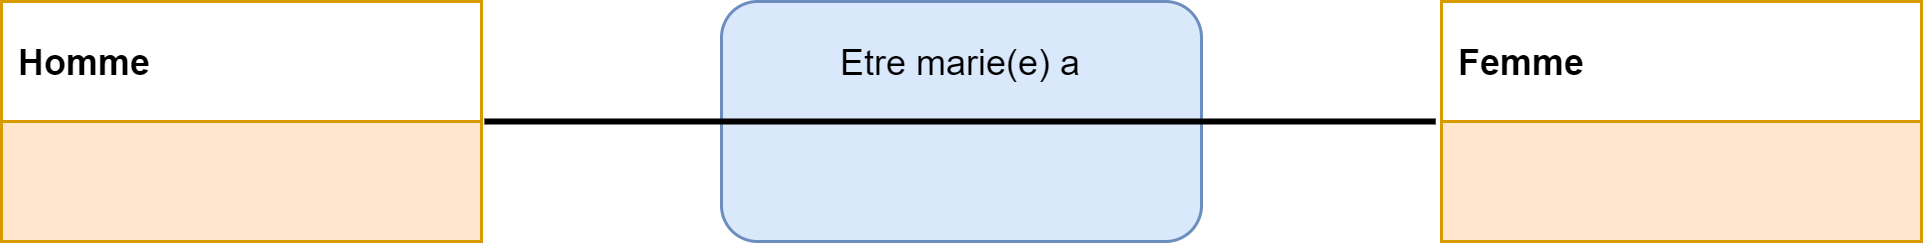
\includegraphics[width=12cm]{img/ex1}
\end{center}
Préciser les cardinalités de l'association \textit{Etre marie(e) a} :
\begin{enumerate}[--]
	\item 	dans une société monogame;
	\item 	dans une société dans laquelle les femmes ont le droit d'être polygames.
\end{enumerate}
\end{exercice}

\begin{exercice}[]
\begin{center}
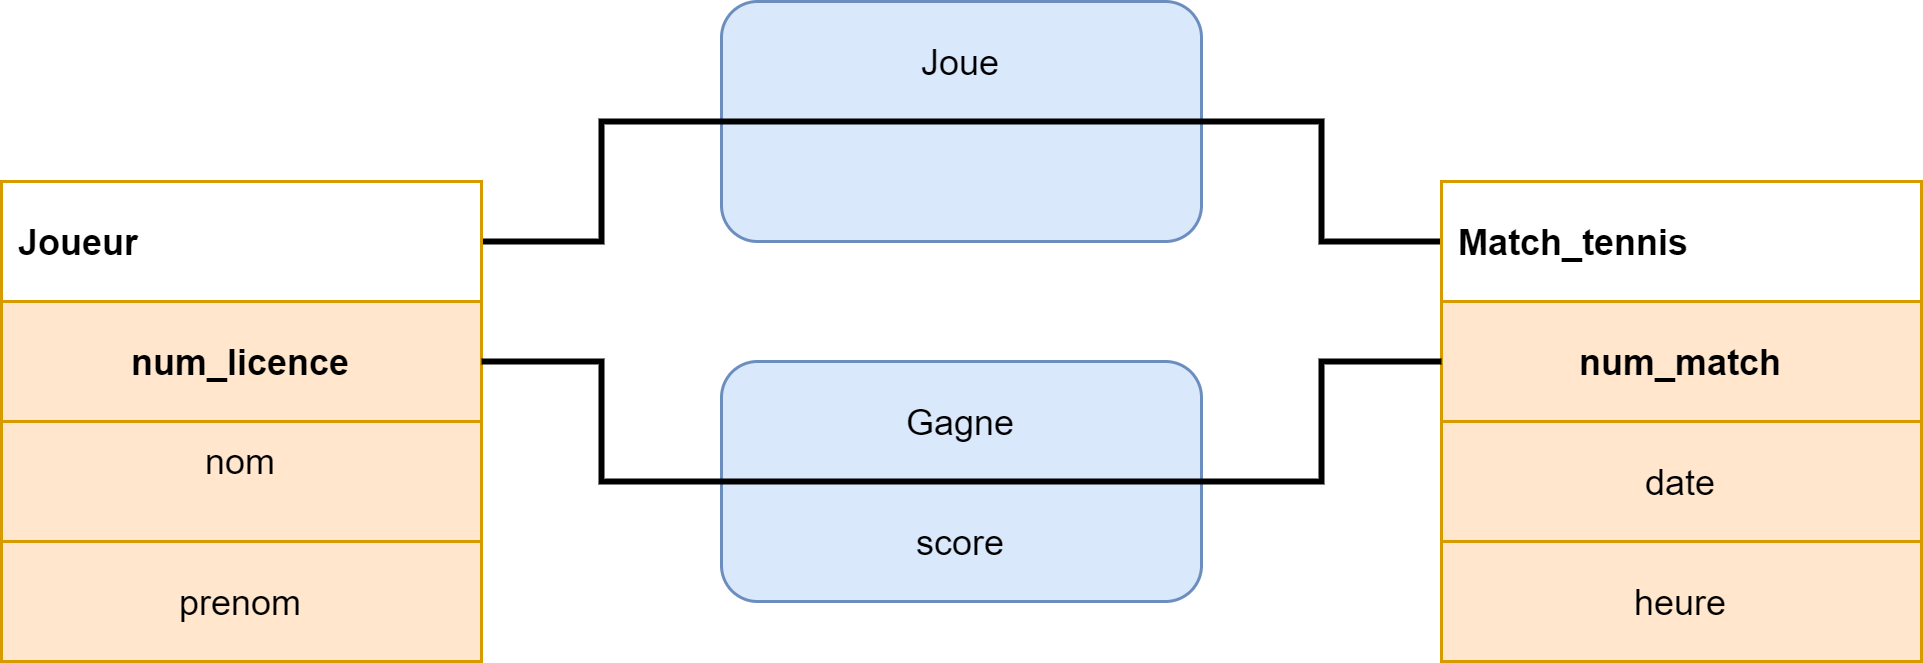
\includegraphics[width=12cm]{img/ex2}
\end{center}
Préciser les cardinalités des associations.
\end{exercice}
\newpage

\begin{exercice}[]
\begin{center}
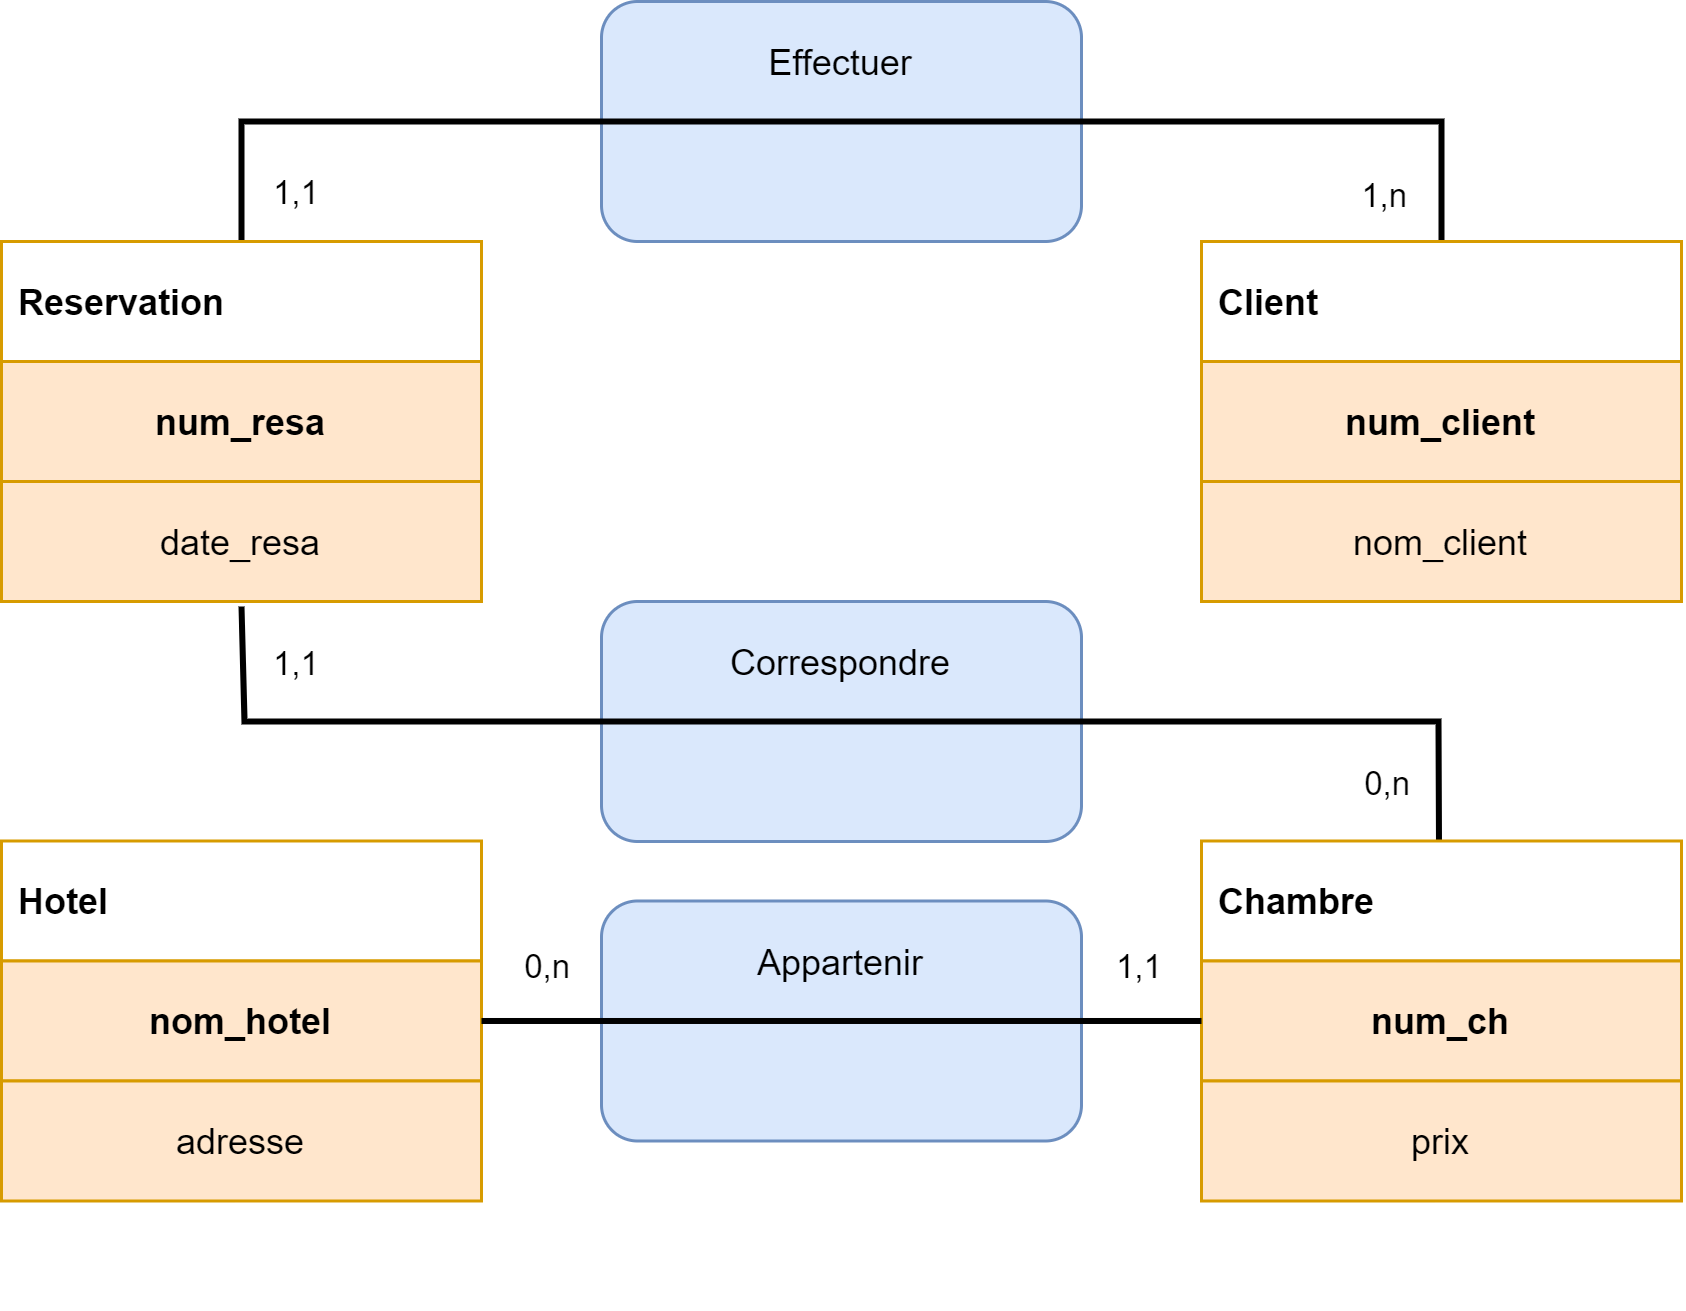
\includegraphics[width=12cm]{img/ex_hotel}
\end{center}
Dans ce modèle
\begin{enumerate}[\bfseries 1.]
	\item 	Peut-on avoir des clients homonymes ?
	\item 	Un client peut-il réserver plusieurs chambres à une même date ?
    \item 	Est-il possible de réserver une chambre plusieurs jours d'affilée ?
    \item 	Peut-on savoir si une chambre est libre à une date donnée ?
    \item 	Peut-on réserver la même chambre plusieurs fois à la même date ?
\end{enumerate}
\end{exercice}
\newpage
\begin{exercice}[]
\begin{center}
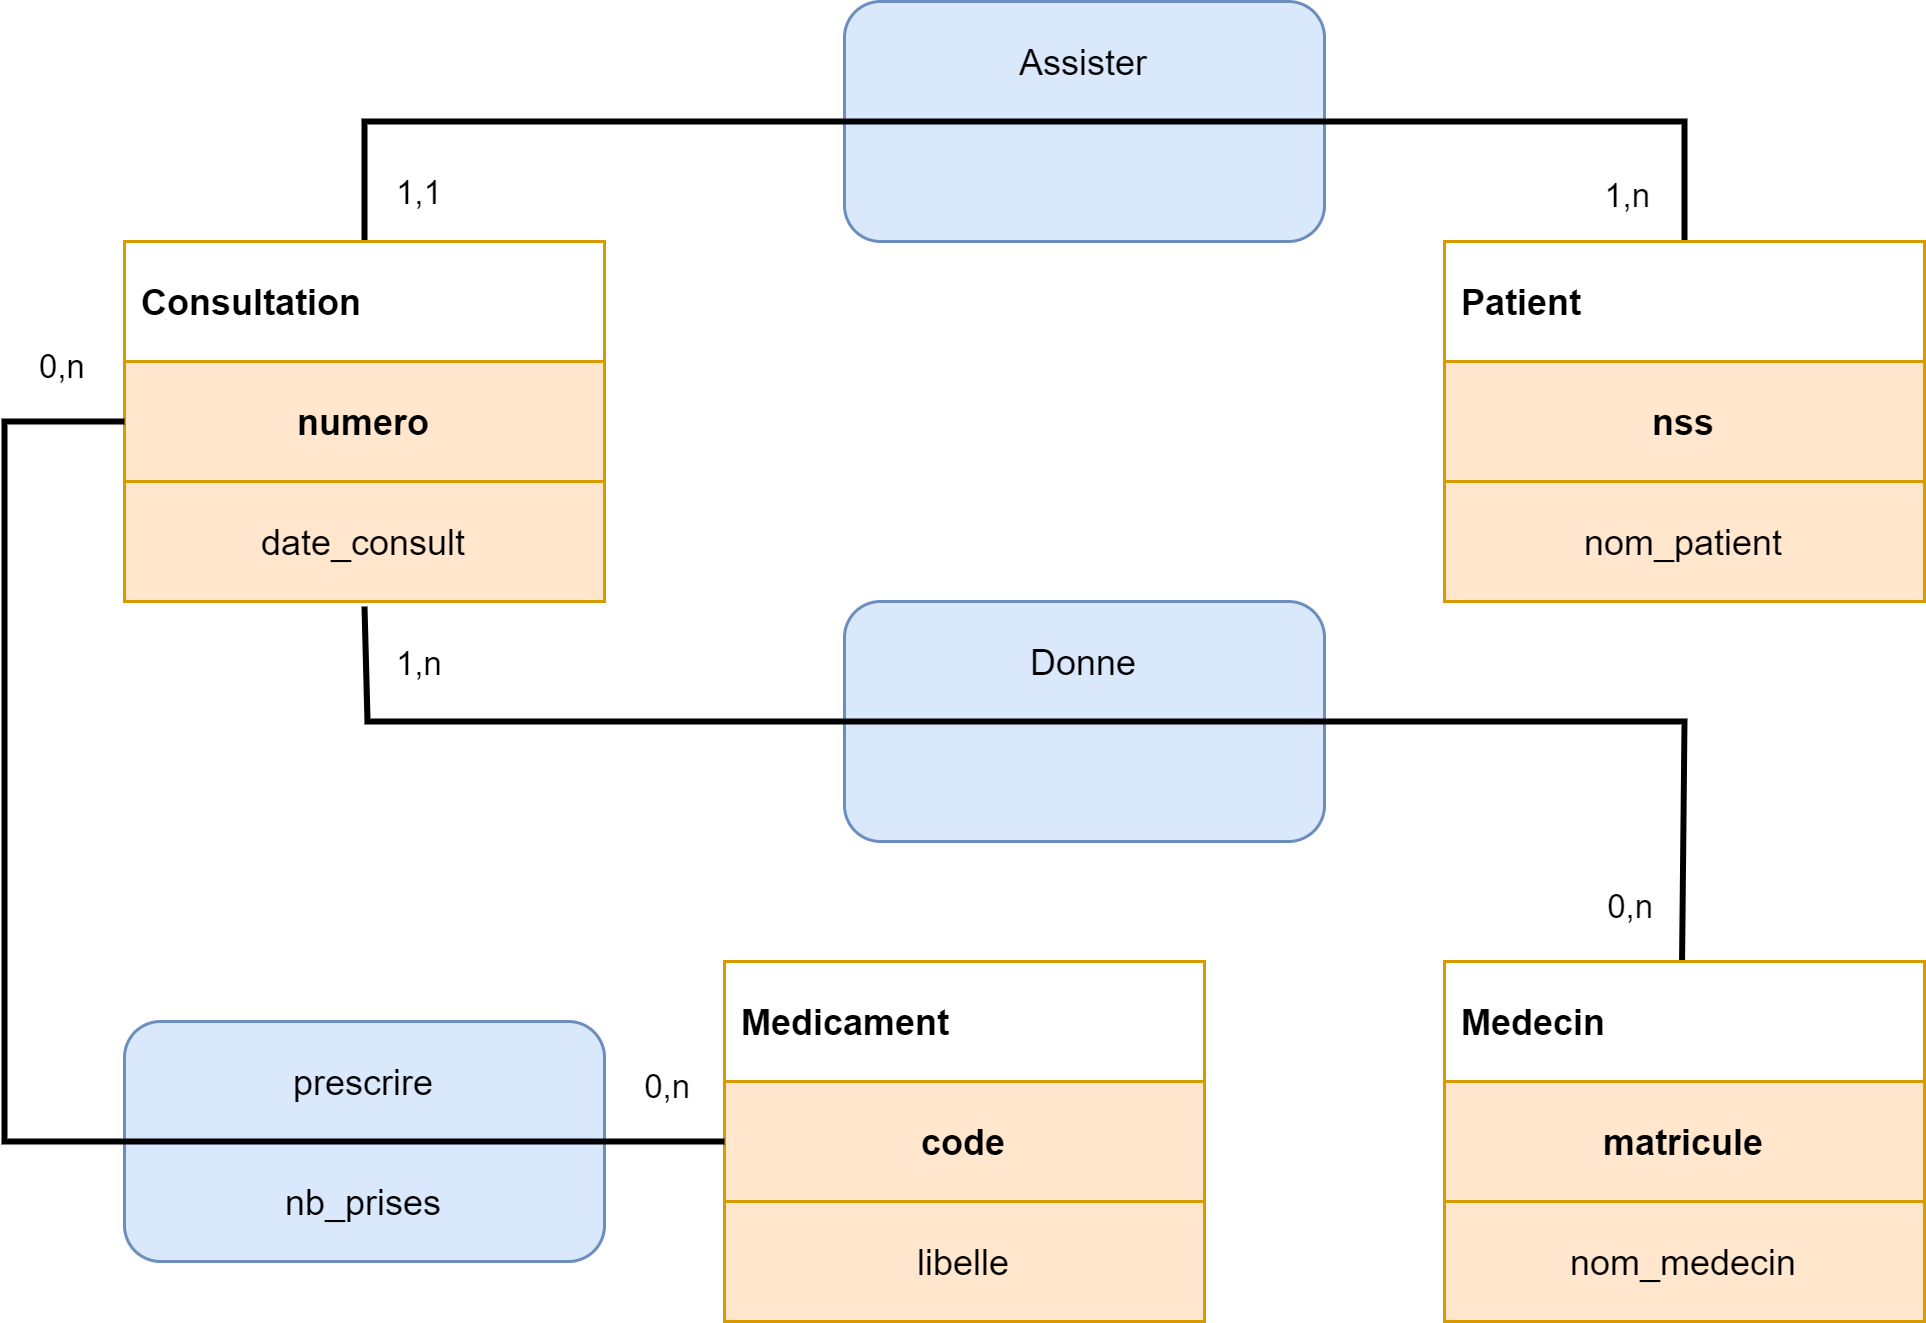
\includegraphics[width=12cm]{img/ex_consultation}
\end{center}
Dans ce modèle
\begin{enumerate}[\bfseries 1.]
	\item 	Un patient peut-il assister à plusieurs consultations ?
    \item   Deux patients peuvent-ils assister à la même consultation ?
    \item   Deux consultations peuvent-elles avoir lieu le même jour ?
	\item 	Un médecin peut-il recevoir plusieurs patients lors d'une même consultation ?
    \item   Plusieurs médecins peuvent-ils assister à la même consultation ?
    \item   Une consultation entraîne-t-elle toujours une prescription ?
    \item 	Peut-on prescrire plusieurs médicaments lors d'une même consultation ?
    \item   Deux médecins différents peuvent-ils prescrire le même médicament ?
    \item   \'Etant donné un médicament prescrit, peut-on toujours connaître le médecin qui l'a prescrit ?

\end{enumerate}
\end{exercice}


\begin{exercice}[]
Une entreprise est identifiée par son nom.\\
Dans cette entreprise, un département est identifié par un nom et caractérisé par une localisation.\\
Un employé est caractérisé par un numéro, son nom, son grade et le département dans lequel il travaille.\\
Le numéro d’un employé est unique dans un département mais pas dans l’entreprise.\\
Donner le MCD, en précisant les attributs.\\

\textit{Indication : \og caractérisé\fg{} fait référence à un attribut, \og identifié\fg{} à un identifiant.}
\end{exercice}

\begin{exercice}[]
\begin{center}
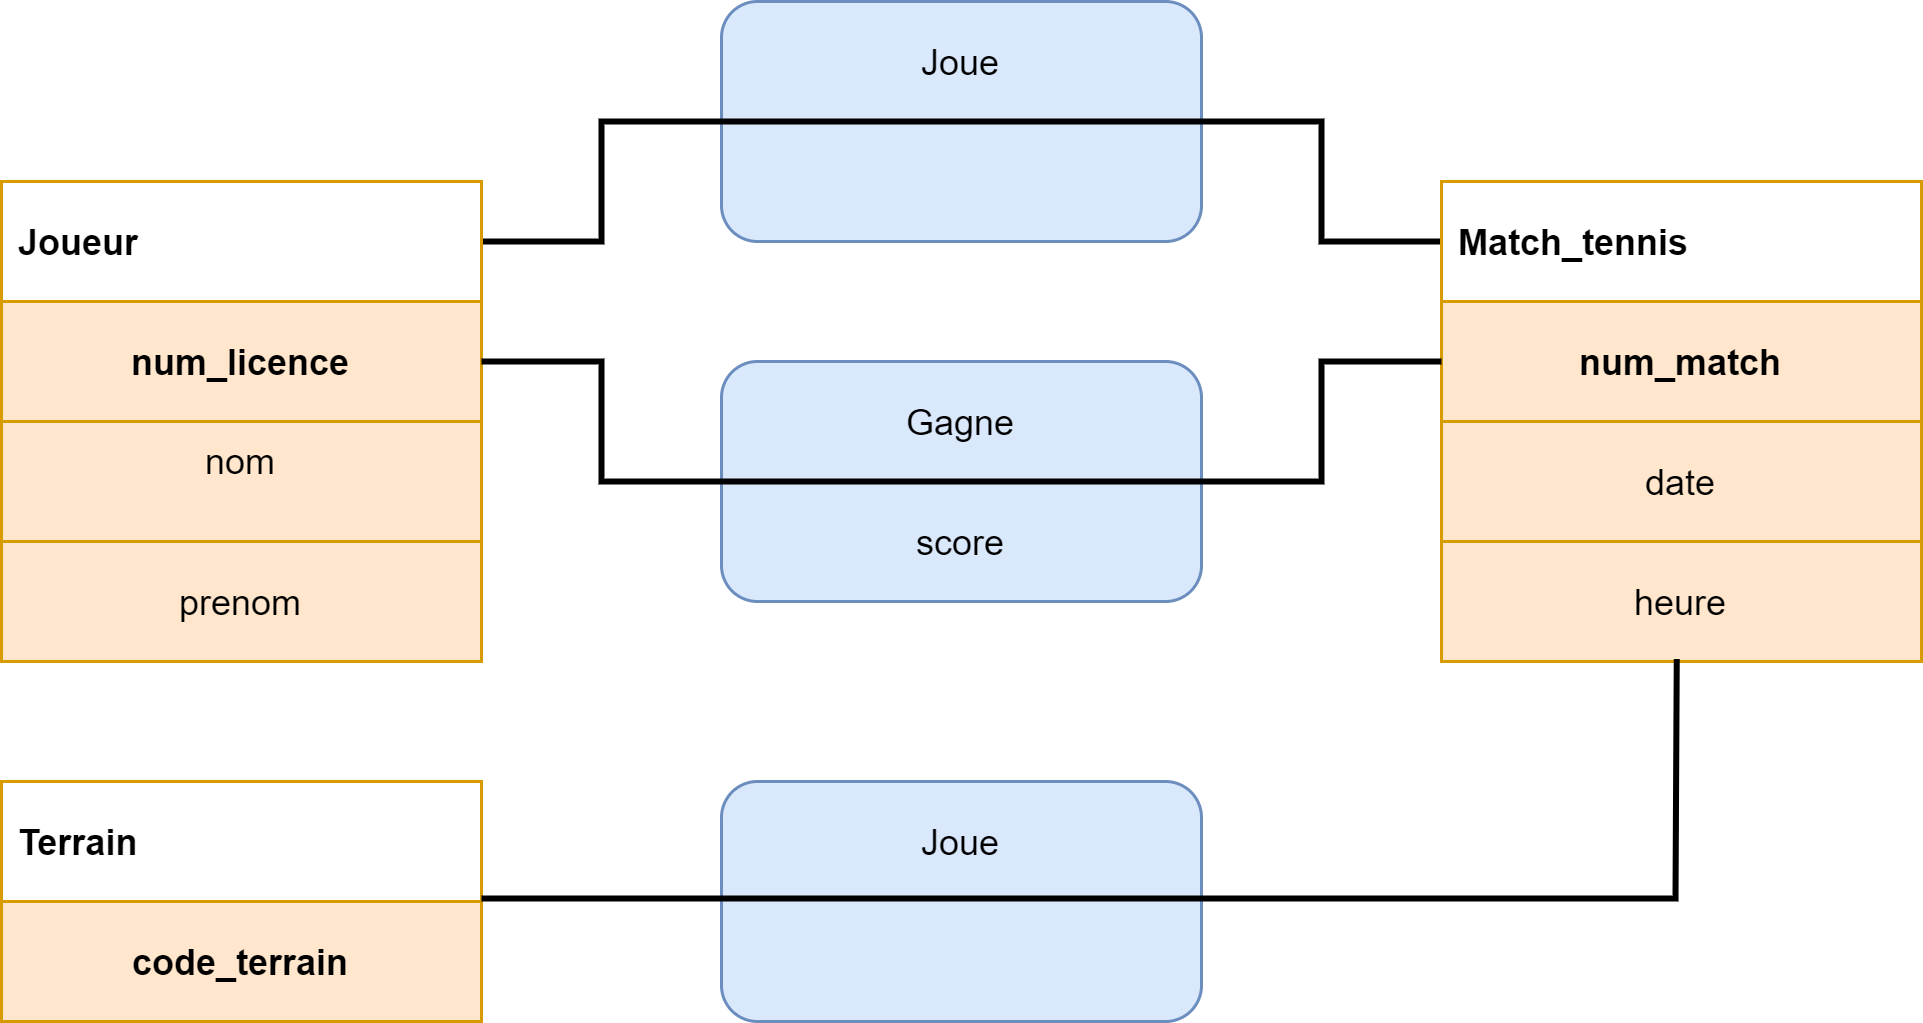
\includegraphics[width=12cm]{img/ex3}
\end{center}
\begin{enumerate}[\bfseries 1.]
	\item 	Reprendre les cardinalités du précédent MCD sur le tennis et préciser celle de \textit{Joue}.
	\item 	Selon ce modèle peut-on jouer des matchs de double ?
    \item 	Un joueur peut-il gagner un match sans y avoir participé ?
    \item 	Peut-il y avoir 2 matchs sur le même terrain à la même heure ?
    \item 	Connaissant un joueur, peut-on savoir sur quel(s) terrain(s) il a joué ?
\end{enumerate}
\end{exercice}

\begin{exercice}[]
On considère une médiathèque contenant des ouvrages pouvant être empruntés.\\
Un ouvrage est caractérisé par un numéro unique, un titre, un auteur et un éditeur. En outre, on décrit un ouvrage par un certain nombre de mots-clés qui indiquent les sujets qui y sont traités.\\
La médiathèque dispose d’un ou plusieurs exemplaires de chaque ouvrage, L’exemplaire est identifié par un numéro et caractérisé par sa position dans les rayonnages et sa date d’achat.
Un exemplaire peut être emprunté par un emprunteur. Ces derniers sont identifiés par un numéro d’emprunteur et possèdent un nom et une adresse.\\

Donner le MCD.
\end{exercice}
\end{document}